\documentclass[]{beamer}
\usepackage{listings}
\usepackage{graphicx}
\usepackage{hyperref}
\usetheme{Antibes}
\usepackage{amsmath}
\usepackage{amsthm}
\usecolortheme{beaver}
\usecolortheme{orchid}
\usecolortheme{whale}
\usepackage{subfig}

\hypersetup{linkcolor=blue, colorlinks=true}

\setbeamerfont{title}{shape=\itshape,family=\rmfamily}


\theoremstyle{definition}
\newtheorem{defn}{Definition}[section]

%\theoremstyle{remark}
%\newtheorem{example}[Example][section]


\title{Better Testing With Bandits}
\author{Paul Gribelyuk}
%\institution{Rakuten Marketing}
\date{\today}

\begin{document}
\frame{\titlepage}

\begin{frame}
	\frametitle{Table of Contents}
	\tableofcontents
\end{frame}


\section{Overview of A/B Testing}


\begin{frame}
	\frametitle{High-Level Overview of A/B Testing - aka Things We Already Know}
	\begin{itemize}
		\item In this lean, "smaller is better", agile new world, we iterate over the Build$\to$Measure$\to$Learn (or MVP$\to$Measure$\to$Pivot) cycle
		\begin{figure}[h!]
		\centering
			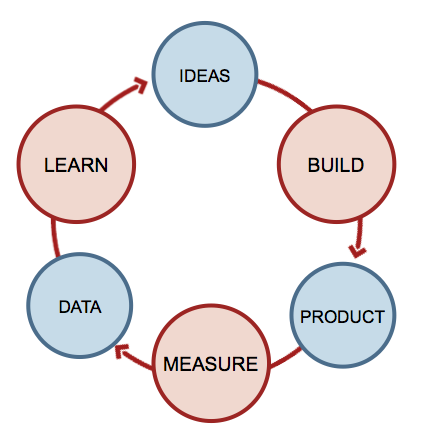
\includegraphics[height=2.5cm]{resources/lean_workflow.png}
		\end{figure}
		\item We choose a metric by which to judge the success of our MVP (e.g. click-through rate, time spent on page, revenue, etc.)
		\item We want to quantify the effect a feature has on the chosen metric.
	\end{itemize}
\end{frame}


\begin{frame}
	\frametitle{A/B Testing, A Definition}

	\begin{defn}<1->[from Wikipedia]
		In marketing, A/B testing is a \emph{simple} randomized experiment with two variants, A and B, which are the control and treatment in the controlled experiment. It is a form of statistical hypothesis testing. Other names include randomized controlled experiments, online controlled experiments, and split testing. \pause\emph{In online settings, such as web design (especially user experience design), the goal is to identify changes to web pages that increase or maximize an outcome of interest (e.g., \textbf{click-through rate} for a banner advertisement)}.
	\end{defn}
	(emphasis mine)
\end{frame}


\begin{frame}
	\begin{figure}[ht!] 
		\centering
		\subfloat[Some Boring Site]{
\includegraphics[width=0.4\linewidth]{resources/google_site.png}}\pause
		\subfloat[I Can Haz Search]{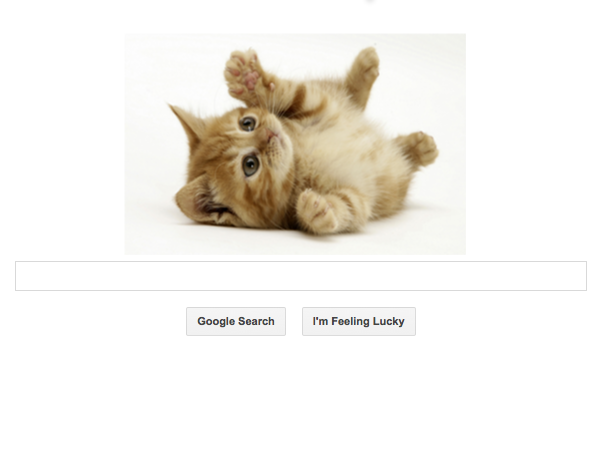
\includegraphics[width=0.4\linewidth]{resources/google_ab_tested.png}}
	\end{figure}

	\begin{figure}
	\centering
		\caption{Progress}
		
\includegraphics[height=2.5cm]{resources/victory_baby.png}
	\end{figure}
\end{frame}


\begin{frame}
	What can we test?\pause
	\begin{itemize}
		\item<2, 9> Affiliate: Change wording, text (font and size), color, placement
		\item<3, 9> Lead Gen: Reorganize a page, remove forms fields, add form fields
		\item<4, 9> Email: Frequency, creative, wording, embedded video, reordering of contents
		\item<5, 9> Display: Change bidding strategy, change interactive nature of ad
		\item<6, 9> Search: Change keywords, change keyword bidding strategy, change search engines used
		\item<7, 9> Any publisher: change composition of displayed ads, sizes, positions, quantities, navigation images
		\item<8, 9> Products: ???
	\end{itemize}
\end{frame}


\begin{frame}
	\begin{example}[Flipping a Coin]
	I put on a Star Wars Tshirt and flip a coin 100 times, getting 48 heads.  Next time, I wear a Star Trek (Original) Tshirt and flip the same coin 100 times, getting 52 heads.  Did I just achieve and 8\% boost in flipping heads?
	\end{example}\pause
	This is a silly example but illustrates the potential pitfalls in claims typically made in marketing materials.
\end{frame}


\begin{frame}	
	The classical testing framework takes the following steps:
	\begin{enumerate}
	\item Specify a null hypothesis: that there is no difference between the two coin-flipping sessions
	\item Make an assumption about the distribution of individual events: $P(heads) = P(tails) = \frac{1}{2}$ and $P(\text{k heads from n flips}) \sim Binomial(k, n)$
	\item Compute the \emph{test statistic} $T = \frac{\bar{x_1} - \bar{x_2}}{\sqrt{(\frac{\sigma_1^2}{n_1} + \frac{s_2^2}{n_2})}}$
	\item Test the hypothesis by considering how likely it is to have generated the test statistic (in our case, $T = 4$).
	\end{enumerate}
	\pause
\end{frame}

\begin{frame}
	\begin{figure}[ht!]
  		\centering
		
\includegraphics[height=7.5cm]{resources/scheduled_program.jpg}
	\end{figure}
\end{frame}


\begin{frame}
	We talked about what we can test, so how do we go about doing it?
	\begin{itemize}[<+->]
		\item Let's collect data about the original (the control) and the feature (the variable) side-by-side
		\item This is how conventional "A/B" testing is done
		\begin{center}
		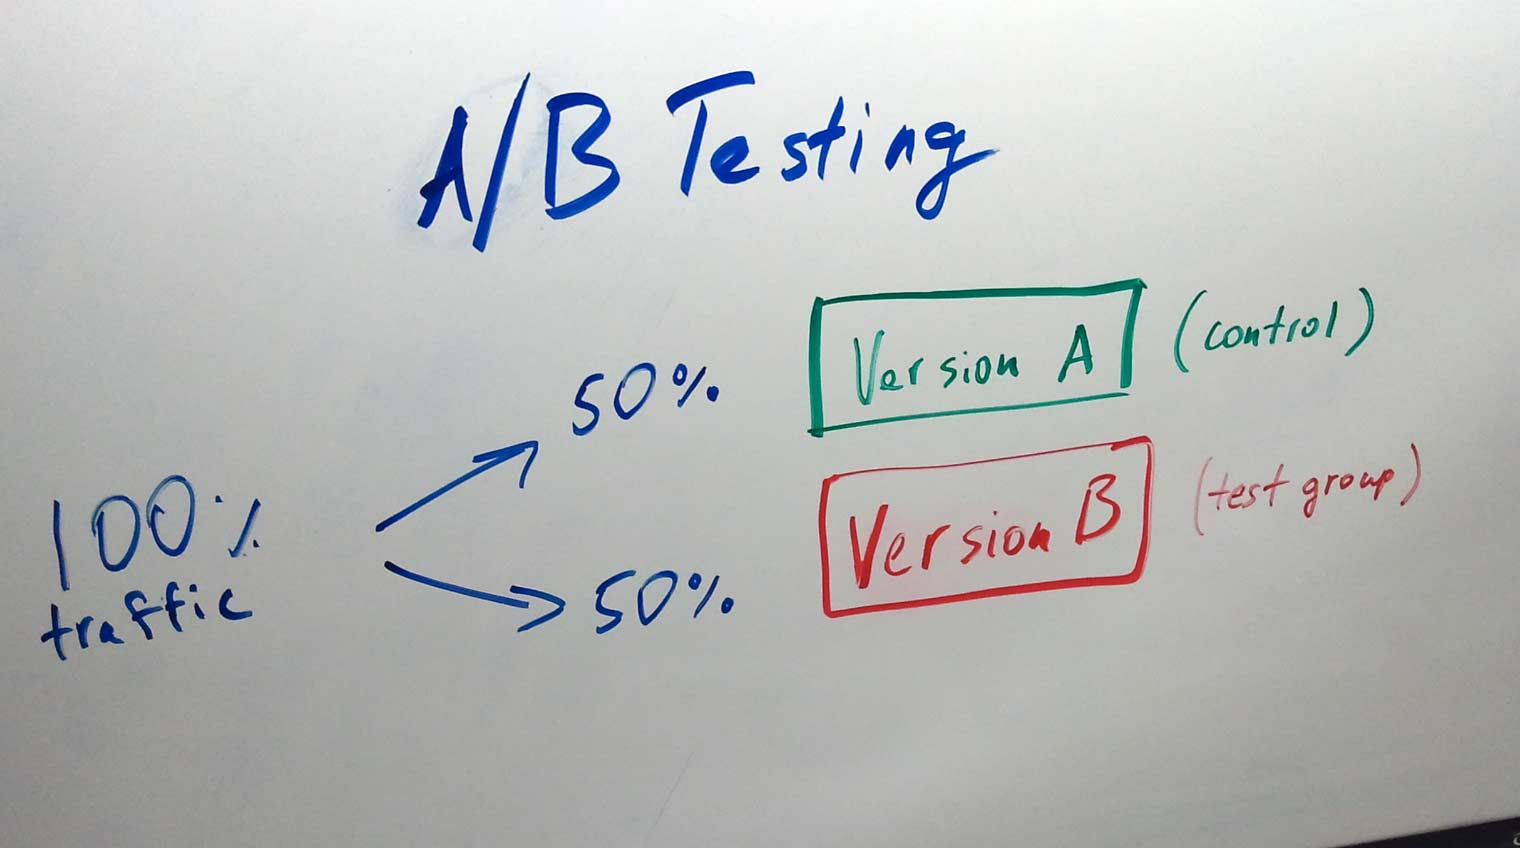
\includegraphics[height=2cm]{resources/ab_testing.jpg}
		\end{center}
		\item When rolling out a major rewrite of an application, this is typically used to measure improvement.  We can start at a 90\%/10\% split and adjust from there according to our performance metric
	\end{itemize}
\end{frame}

%\begin{frame}
%Example - Google Maps
%\begin{figure}[ht!] 
%\centering
%\subfloat{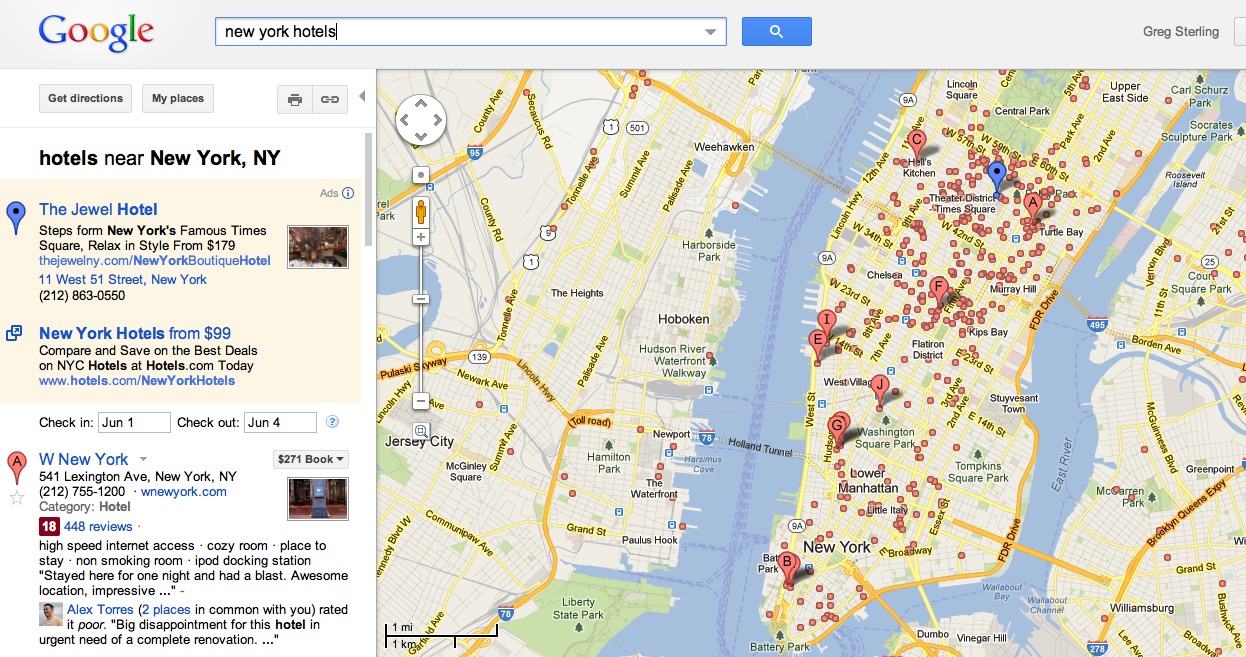
\includegraphics[width=0.38\linewidth]{resources/google_maps_old.png}}
%\subfloat{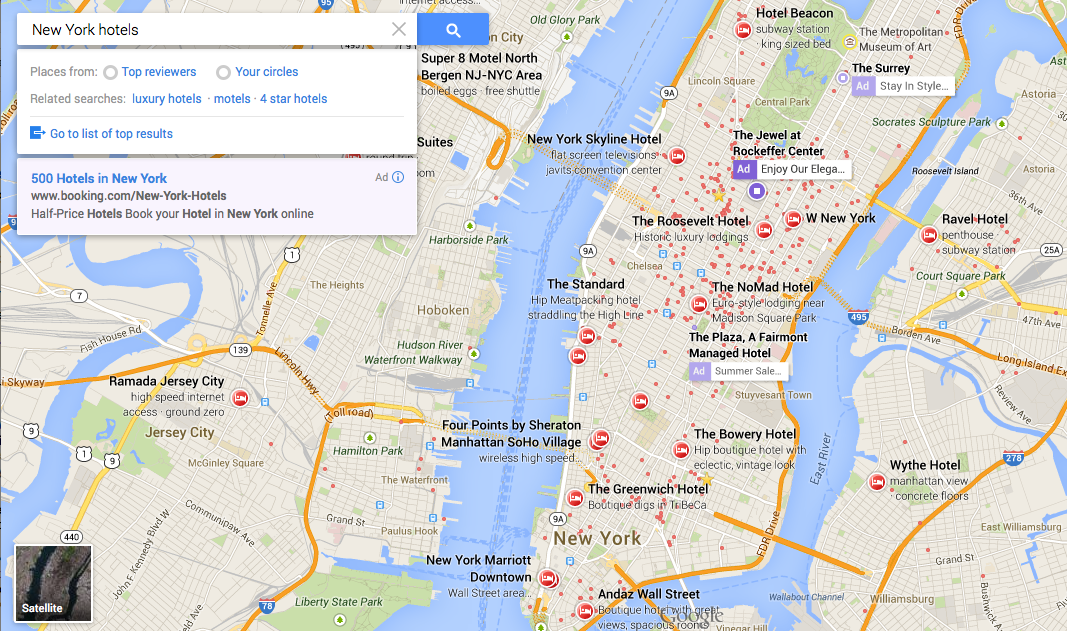
\includegraphics[width=0.38\linewidth]{resources/google_maps_new.png}}
%\caption{Google Maps Before and After}
%\end{figure}
%\pause
%\begin{figure}[ht!] 
%\centering
%\subfloat{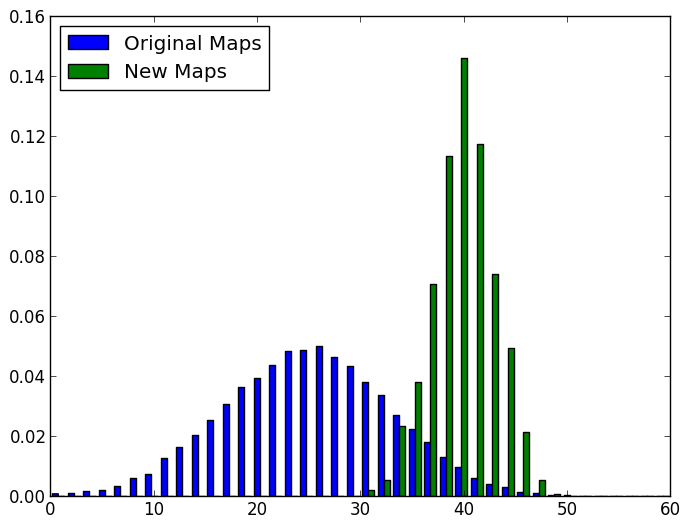
\includegraphics[height=2.6cm]{resources/ab_test_result2.png}}
%\caption{Hypothetical Measured Time Spent on Both Sites}
%\end{figure}
%\end{frame}

\subsection{How To Measure Performance?}

\begin{frame}
Examples of Useful Performance Measures:
\begin{description}
\item[Site Redesign] Avg. Time Spent, Degree of Site Exploration (percentage of links clicked)
\item[Mailing List Format] Clickthrough Rate, Forwarding Rate
\item[Product Description] \$ Revenue
\end{description}
%For the last item, we can start to see where A/B testing can fall over.  Specifically, when we start to introduce more than just two variants, we immediately need significantly more data to gain certainty about our prediction

In each case, we run some form of a t-test test to determine whether the feature had a statistically-significant impact on the measure we are trying to optimize
\end{frame}

\begin{frame}
We will need a bit of math to demonstrate the limitations of conventional A/B testing:
\begin{theorem}[Central Limit Theorem]
If $X_i$ are normal independently distributed variables with mean $\mu$ and variance $\sigma^2$ and $S_n = \frac{1}{n}\sum_{i=1}^n X_i$, then $S_n$ has mean $\mu$ and variance $n\sigma^2$ 
\end{theorem}
Thus, if we make these (strong) assumptions about the distribution of the measurements of feature A and feature B, then we can see that to double our confidence in the conclusion, we would need to quadruple the number of samples.
\end{frame}

\subsection{Demo}

%\begin{frame}
%\frametitle{An Aside About Probability Distributions}
%\begin{itemize}
%\item Normal distributions (thin tail) occur frequently in many naturally occuring physical phenomena such as the dissipation of heat, rolls of a fair dice, etc.
%\item The Poisson distribution is better suited at explaining random arrival times of customers (in supermarkets, networks)
%\item Power-law (fat-tail or Levy) distributions are more suited at explaining events linked to human behavior:
%\begin{itemize}
%\item Accumulation of Wealth
%\item Hurricane Intensities
%\item Book Sales, Success of Football Players and Musicians, Youtube views, Twitter followers, etc.
%\end{itemize}
%\item Others: Gamma, Beta, Dirichlet\ldots
%\end{itemize}
%The fatter the tail, the longer it takes to estimate parameters such as mean and variance.
%\end{frame}

\subsection{Scaling to A/B/C/... Testing}
\begin{frame}
\frametitle{What if we wanted to test many?}
\begin{figure}[ht!] 
\centering
\subfloat{
\includegraphics[width=0.35\linewidth]{resources/google_site1.png}}\pause
\subfloat{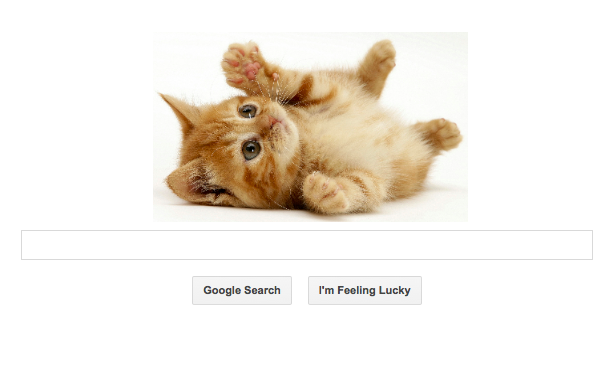
\includegraphics[width=0.35\linewidth]{resources/google_site2.png}}\pause\\
\subfloat{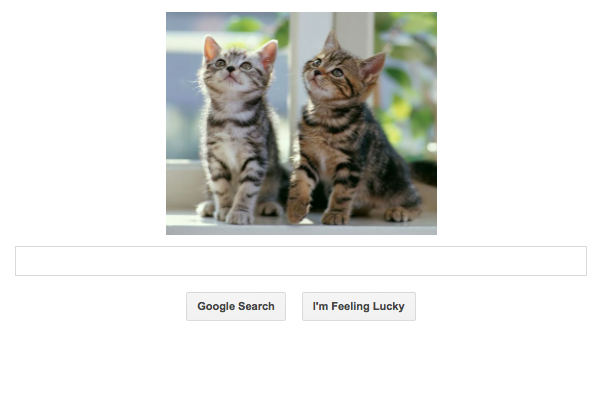
\includegraphics[width=0.35\linewidth]{resources/google_site3.png}}\pause
\subfloat{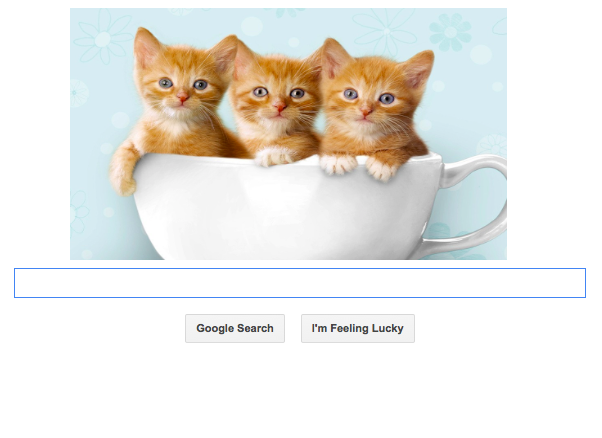
\includegraphics[width=0.35\linewidth]{resources/google_site4.png}}
\caption{Which one will the users love the most?}
\end{figure}
\end{frame}


\begin{frame}
\frametitle{Outline of Process}
We will label the versions by the number of cats they have: $C_0, C_1, C_2, C_3, \ldots C_n$
\begin{enumerate}[<+->]
\item  Run A/B test for $C_0$ vs $C_1$, the winner becomes the new control, $C_{control}$
\item Run A/B test for $C_{control}$ vs $C_2$, the winner becomes new control $C_{control}$
\item ad infinatum
\end{enumerate}
Note that at each turn we are wasting valuable time and potentially losing users due to an inferior number of cats.  Alternatively, we could run them all side-by-side, but it would take just as many points to attain \emph{statistical significance} as specified by our test statistics and the CLT.
\end{frame}


\section{Exploration vs Exploitation}
\subsection{The $\epsilon$-Greedy Approach}
\begin{frame}
\frametitle{Greedy Algorithms}
\begin{figure}[h!]
\centering
	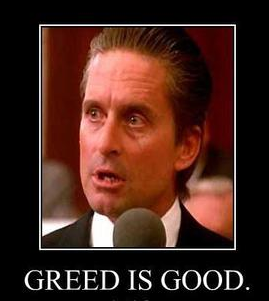
\includegraphics[height=2.5cm]{resources/greedisgood.png}
\end{figure}	
\ldots well, it's definitely \emph{better}
\begin{defn}[Wikipedia to the rescue]
A greedy algorithm is an algorithm that follows the problem solving heuristic of making the locally optimal choice at each stage with the hope of finding a global optimum. In many problems, a greedy strategy does not in general produce an optimal solution
\end{defn}
\end{frame}


\begin{frame}
\frametitle{$\epsilon$-greedy}
We are now in the world of bandit strategies!  The idea is that we run the $C_0/C_1/C_2/\ldots$ versions side-by-side in the following way:
\begin{enumerate}
\item Initialize all variants to be equally likely to be selected for display for a user (i.e. if we have 10 of them, each one gets chosen with $p = 0.1$)
\item Keep track of the running performance of all the variants 
\item Choose the best one with probability $1 - \epsilon$
\item Choose equally from all the variants with probability $\epsilon$
\item Break ties by choosing randomly, or one with the lowest ID, etc.
\item Rinse and repeat until a clear winner emerges.
\end{enumerate}
\end{frame}


\subsection{How To Choose $\epsilon$?}
\begin{frame}
\frametitle{Exploration vs Exploitation}
\onslide<1, 3>{Every time we are \emph{greedy}, we are displaying the winner, i.e. \textbf{exploiting} what we have learned about the environment we are in.}
\onslide<2, 3>{The rest of the time, we choose to pick uniformly from the available bandits, i.e. \textbf{exploring} the environment to gain more familiarity (statistical confidence)}
\onslide<3>{This is a technique more generally used in robotics, where a robot senses (explores) its environment and then acts (exploits) based on the obtained knowledge.  This technique is the basis for learning unfamiliar environments (think Google driverless cars), as well as path planning (what is the optimal route between two points in this paritially-unfamiliar environment?).}
\end{frame}


\subsection{Demo}
\subsection{Other Approaches}
\begin{frame}
Within the $\epsilon$-greedy framework, we could improve the performance if we know something about the data:
\begin{itemize}[<+->]
\item $\epsilon$-first Start by exploring only, then switch to exploiting; if there are $N$ visitors to the site, begin with $\epsilon N$ exploration steps followed by $(1 - \epsilon)N$ exploitation steps 
\item $\epsilon$-decreasing Start with a high $\epsilon$, and gradually reduce it to 0 over time.
\item $\epsilon$-adaptive: Adapt $\epsilon$ base on how much the performance values are fluctuating (variance)
\item More, a field of active research
\end{itemize}
\end{frame}


\section{Multi-Armed Bandits}
\subsection{Motivation}
\begin{frame}
\frametitle{Can We Do Better?  Lerning to Live with Regret}
\begin{defn}[Regret]
The regret incurred by a specific strategy is the difference between the optimal strategy (only known in hindsight) and that strategy.  More formally, if we have $N$ rounds ($N$ users hitting the site)
$$
\rho = N\mu^{*} - \sum_{i=1}^N\hat{r}_i
$$
with $\mu^*$ representing the (unknown) optimal strategy and $\hat{r}_i$ is the reward from our chosen strategy at a given time $i$.
\end{defn}
It's clear that A/B testing does not minimize regret since we wind up alienating a lot of users during our discovery process.  It's also clear that $\epsilon$-greedy strategies are better, but by how much?
\end{frame}
\subsection{Demo}


\subsection{Background on Beta Distribution}
\begin{frame}
\frametitle{How I Stopped Worrying and Learned to Love the Beta Distribution}
\begin{defn}[Beta Distribution]
This is a two-parameter probability distribution over the interval $[0, 1]$, and because of this, it is used to model "the probability of probabilities".  The two parameters are labeled $\alpha$ and $\beta$ and skew the density function either to the left (higher $\alpha$) or to the right (higher $\beta$).  The density function is written as:
$$
Beta_{\alpha, \beta}(x) \sim x^{\alpha - 1}(1 - x)^{\beta - 1}
$$
\end{defn}\pause
\end{frame}


\begin{frame}
\frametitle{Pictorially}
\begin{figure}[ht!] 
\centering
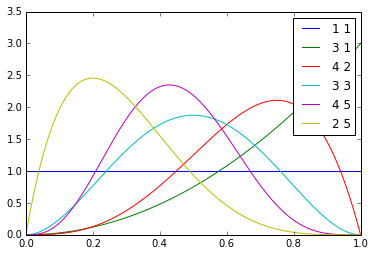
\includegraphics[width=0.7\linewidth]{resources/alpha_beta_charts.png}
\caption{Examples of Different $\alpha$ and $\beta$ values}
\end{figure}

Why do we need this mess?

\end{frame}


\subsection{Algorithm}
\begin{frame}
\frametitle{Bandits Algorithm - Thompson Sampling}
\begin{itemize}[<+->]
\item Initialize each bandit with its very own Beta distribution with parameters $\alpha = 1$ and $\beta = 1$ (the uniform distribution).
\item In the context of testing performance, $\alpha$ represents number of conversions and $\beta$ represents number of non-conversions
\item In each round:
\begin{itemize}
	\item Sample from each of the Beta distributions and pick the bandit which produced the highest value
	\item Serve the corresponding site
	\item If the bandit succeeds at conversion, update $\alpha$ by 1, otherwise, update $\beta$ by 1
\end{itemize}
\item ???
\item Profit - e.g. mathematically proven to minimize regret!!!
\end{itemize}
\end{frame}
\subsection{Resources}

\begin{frame}
\frametitle{Further Reading - Links to Resources}
\begin{itemize}
\item \href{http://20bits.com/article/statistical-analysis-and-ab-testing}{Statistical Analysis and A/B Testing}
\item \href{http://www.amazon.com/Reinforcement-Learning-Introduction-Adaptive-Computation/dp/0262193981}{Reinforcement Learning book}
\item \href{http://www.socialresearchmethods.net/selstat/ssstart.htm}{Selecting Statistical Tests}
\item \href{http://www.graphpad.com/support/faqid/1790/}{Background on Statistical Tests}
\item \href{http://www.meetup.com/NYData/events/160722942/?_af_eid=160722942&a=uc1_te&_af=event}{Meetup Event}
\item \href{http://chrishalpert.com/NYDW\%20Bandit\%20Presentation.ppsx}{Meetup Event Slides}
\end{itemize}
\end{frame}


\end{document}